\documentclass[a4paper,12pt,oneside]{article}
\usepackage{graphicx}
\usepackage{hyperref}
\usepackage[T1]{fontenc}
\usepackage[utf8]{inputenc}
\usepackage{setspace}
\usepackage{amsmath}
\usepackage{amssymb}
\usepackage{tikz}
\usepackage{forest}

\usepackage{mathtools}
\DeclarePairedDelimiter\ceil{\lceil}{\rceil}
\DeclarePairedDelimiter\floor{\lfloor}{\rfloor}

\begin{document}

\thispagestyle{plain}
\begin{center}
  \normalsize
  \textbf{Assignment 3}
  
  \vspace{0.2cm}
  \normalsize
  12/11/2022
  
  \vspace{0.2cm}
  \textbf{Francesco Refolli 865955}
\end{center}

\section{Esercizio 1}

\paragraph{Consegna}

Una catena di supermercati deve decidere quali tra 5 dei suoi magazzini aprire per rifornire 10 nuovi punti vendita. Il costo per l’apertura e mantenimento del magazzino i e' di $\theta_i$ euro. In ciascun magazzino i possono essere stoccati $\alpha_i$ Kg di merce. Ciascun supermercato j si aspetta giornalmente di ricevere almeno $\beta_j$ Kg di merce. Il costo di trasporto unitario di trasporto della merce dal magazzino i al punto vendita j è stimato a $y_{ij}$ euro/Kg. Elaborare un modello di Programmazione Lineare Intera che aiuti la catena di supermercati a decidere quali magazzini aprire e a soddisfare le domande dei punti vendita, minimizzando i costi totali.
Si tenga inoltre in considerazione che la catena:
\begin{enumerate}
\item vuole aprire al massimo 4 magazzini
\item per ragioni logistiche, vuole aprire il magazzino 5 solo se il magazzino 4 e il magazzino 3 non vengono aperti
\item impone che il magazzino 1 consegni la merce al supermercato 5 (il più distante) solo in pallet da $k$ kg (si supponga che $a_i$ sia multiplo di k)
\item vuole che almeno uno dei seguenti scenari sia verificato: scenario a) siano aperti almeno 3 magazzini scenario b) sia aperto almeno 1 tra i magazzini 1, 2 e 5.
\end{enumerate}

\paragraph{Modello - funzione obiettivo}
$d_{ij}$ e' la quantita' di prodotto intera mandata dal magazzino $i$ al supermercato $j$.
\begin{align*}
  min & \Sigma ^ {5} _ {i=1} \Sigma ^ {10} _ {j=1} d_{ij} \cdot y_{ij} & funzione \;\; obiettivo \\
  d_{ij} &\geq 0 \; e \;\; intera & \forall i,j \in [1,5] x [1,10]
\end{align*}

\paragraph{Modello - vincoli di coerenza del problema di trasporto}
\begin{align*}
  \Sigma ^ {10} _ {j} d_{ij} &\leq a_{i} & \forall i \in [1,5] \\
  \Sigma ^ {5} _ {i} d_{ij} &= b_{j} & \forall j \in [1,10]
\end{align*}

\paragraph{Modello - condizione 1}

Si vuole aprire al massimo 4 magazzini. Sfrutto la ricetta \textbf{Vincoli di tipo Either-Or}.
Con $M$ variabile con valore enorme di supporto per le variabili binarie $v_i$ create e necessarie alla condizione 1.

\begin{align*}
  \Sigma ^ {10} _ {j=1} d_{ij} &\leq 0 + M \cdot v_i & \forall i [1,5] \\
  \Sigma ^ {10} _ {j=1} d_{ij} &\geq 1 - M \cdot (1 - v_i) & \forall i [1,5] \\
  \Sigma ^ {5} _ {i=1} v_i &\leq 4 \; e \;\; intera \\
  v_i &\geq 0 \; e \;\; intera & \forall i \in [1,5] \\
  v_i &\leq 1 \; e \;\; intera & \forall i \in [1,5]
\end{align*}

\paragraph{Modello - condizione 2}
Si vuole aprire il magazzino 5 solo se il magazzino 4 e il magazzino 3 non vengono aperti.
Sfrutto la ricetta \textbf{Vincoli di tipo Either-Or}.
Con $M$ variabile con valore enorme di supporto per la variabile binaria $u$ creata e necessaria alla condizione 2.

\begin{align*}
  \Sigma ^ {10} _ {j=1} d_{5j} &\leq 0 + M \cdot u \\
  \Sigma ^ {10} _ {j=1} d_{3j} &\geq 0 - M \cdot u \\
  \Sigma ^ {10} _ {j=1} d_{4j} &\geq 0 - M \cdot u \\
  \Sigma ^ {10} _ {j=1} d_{5j} &\geq 1 - M \cdot (1 - u) \\
  \Sigma ^ {10} _ {j=1} d_{3j} &\leq 0 + M \cdot (1 - u) \\
  \Sigma ^ {10} _ {j=1} d_{4j} &\leq 0 + M \cdot (1 - u) \\
  u &\geq 0 \; e \;\; intera \\
  u &\leq 1 \; e \;\; intera
\end{align*}

\paragraph{Modello - condizione 3}
Si impone che il magazzino 1 consegni la merce al supermercato 5 (il più distante) solo in pallet da $k$ kg.
x e' la quantita' di pallet che il magazzino 1 spedisce al supermercato 5.
\begin{align*}
  d_{ij} - k \cdot x &= 0 \\
  x &\geq 0 \; e \;\; intera
\end{align*}

\paragraph{Modello - condizione 4}
Si vuole che almeno uno dei seguenti scenari sia verificato: scenario a) siano aperti almeno 3 magazzini scenario b) sia aperto almeno 1 tra i magazzini 1, 2 e 5. Sfrutto la ricetta \textbf{K Vincoli su N}.
Con $M$ variabile dal valore enorme e $N = ~ 2 \cdot M$.

\begin{align*}
  \Sigma ^ {10} _ {j=1} d_{ij} &\leq 0 + M \cdot s_i + N \cdot t_1 & \forall i [1,5] \\
  \Sigma ^ {10} _ {j=1} d_{ij} &\geq 1 - M \cdot (1 - s_i) - N \cdot t_1 & \forall i [1,5] \\
  \Sigma ^ {5} _ {i=1} s_i &\geq 3 \\
  \Sigma ^ {10} _ {j=1} d_{1j} &\geq 1 - N \cdot t_2 \\
  \Sigma ^ {10} _ {j=1} d_{2j} &\geq 1 - N \cdot t_3 \\
  \Sigma ^ {10} _ {j=1} d_{5j} &\geq 1 - N \cdot t_4 \\
  \Sigma ^ {4} _ {l=1} t_l &\leq 3 \\
  t_i &\geq 0 \; e \;\; intera & \forall i \in [1,4] \\
  t_i &\leq 1 \; e \;\; intera & \forall i \in [1,4] \\
  s_i &\geq 0 \; e \;\; intera & \forall i \in [1,5] \\
  s_i &\leq 1 \; e \;\; intera & \forall i \in [1,5]
\end{align*}

\newpage
\section{Esercizio 2}

Trovare l’ottimo del seguente problema di Programmazione Lineare Intera applicando l’algoritmo di Branch \& Bound, adottando una tecnica di esplorazione dell’albero Depth First (con navigazione a sinistra). Riportare l’albero di ricerca ottenuto, evidenziando chiaramente l’ordine di esplorazione dei nodi, i branching effettuali, i criteri di fathoming eventualmente applicati, la soluzione ottima e il valore ottimo del rilassamento continuo in ogni nodo. Risolvere tutti i rilassamenti continui per via grafica, mostrando la regione ammissibile iniziale e come essa cambi con l’aggiunta dei vincoli di branching.

\begin{align*}
  max & 2 x_1 + x_2 \\
  5 x_1 + 3 x_2 &\leq 9 \\
  4 x_1  - 3 x_2 &\leq 3 \\
  x_1,x_2 &\geq \;\; e \;\; intere
\end{align*}

\newpage
\paragraph{Passo 1}
\begin{center}
        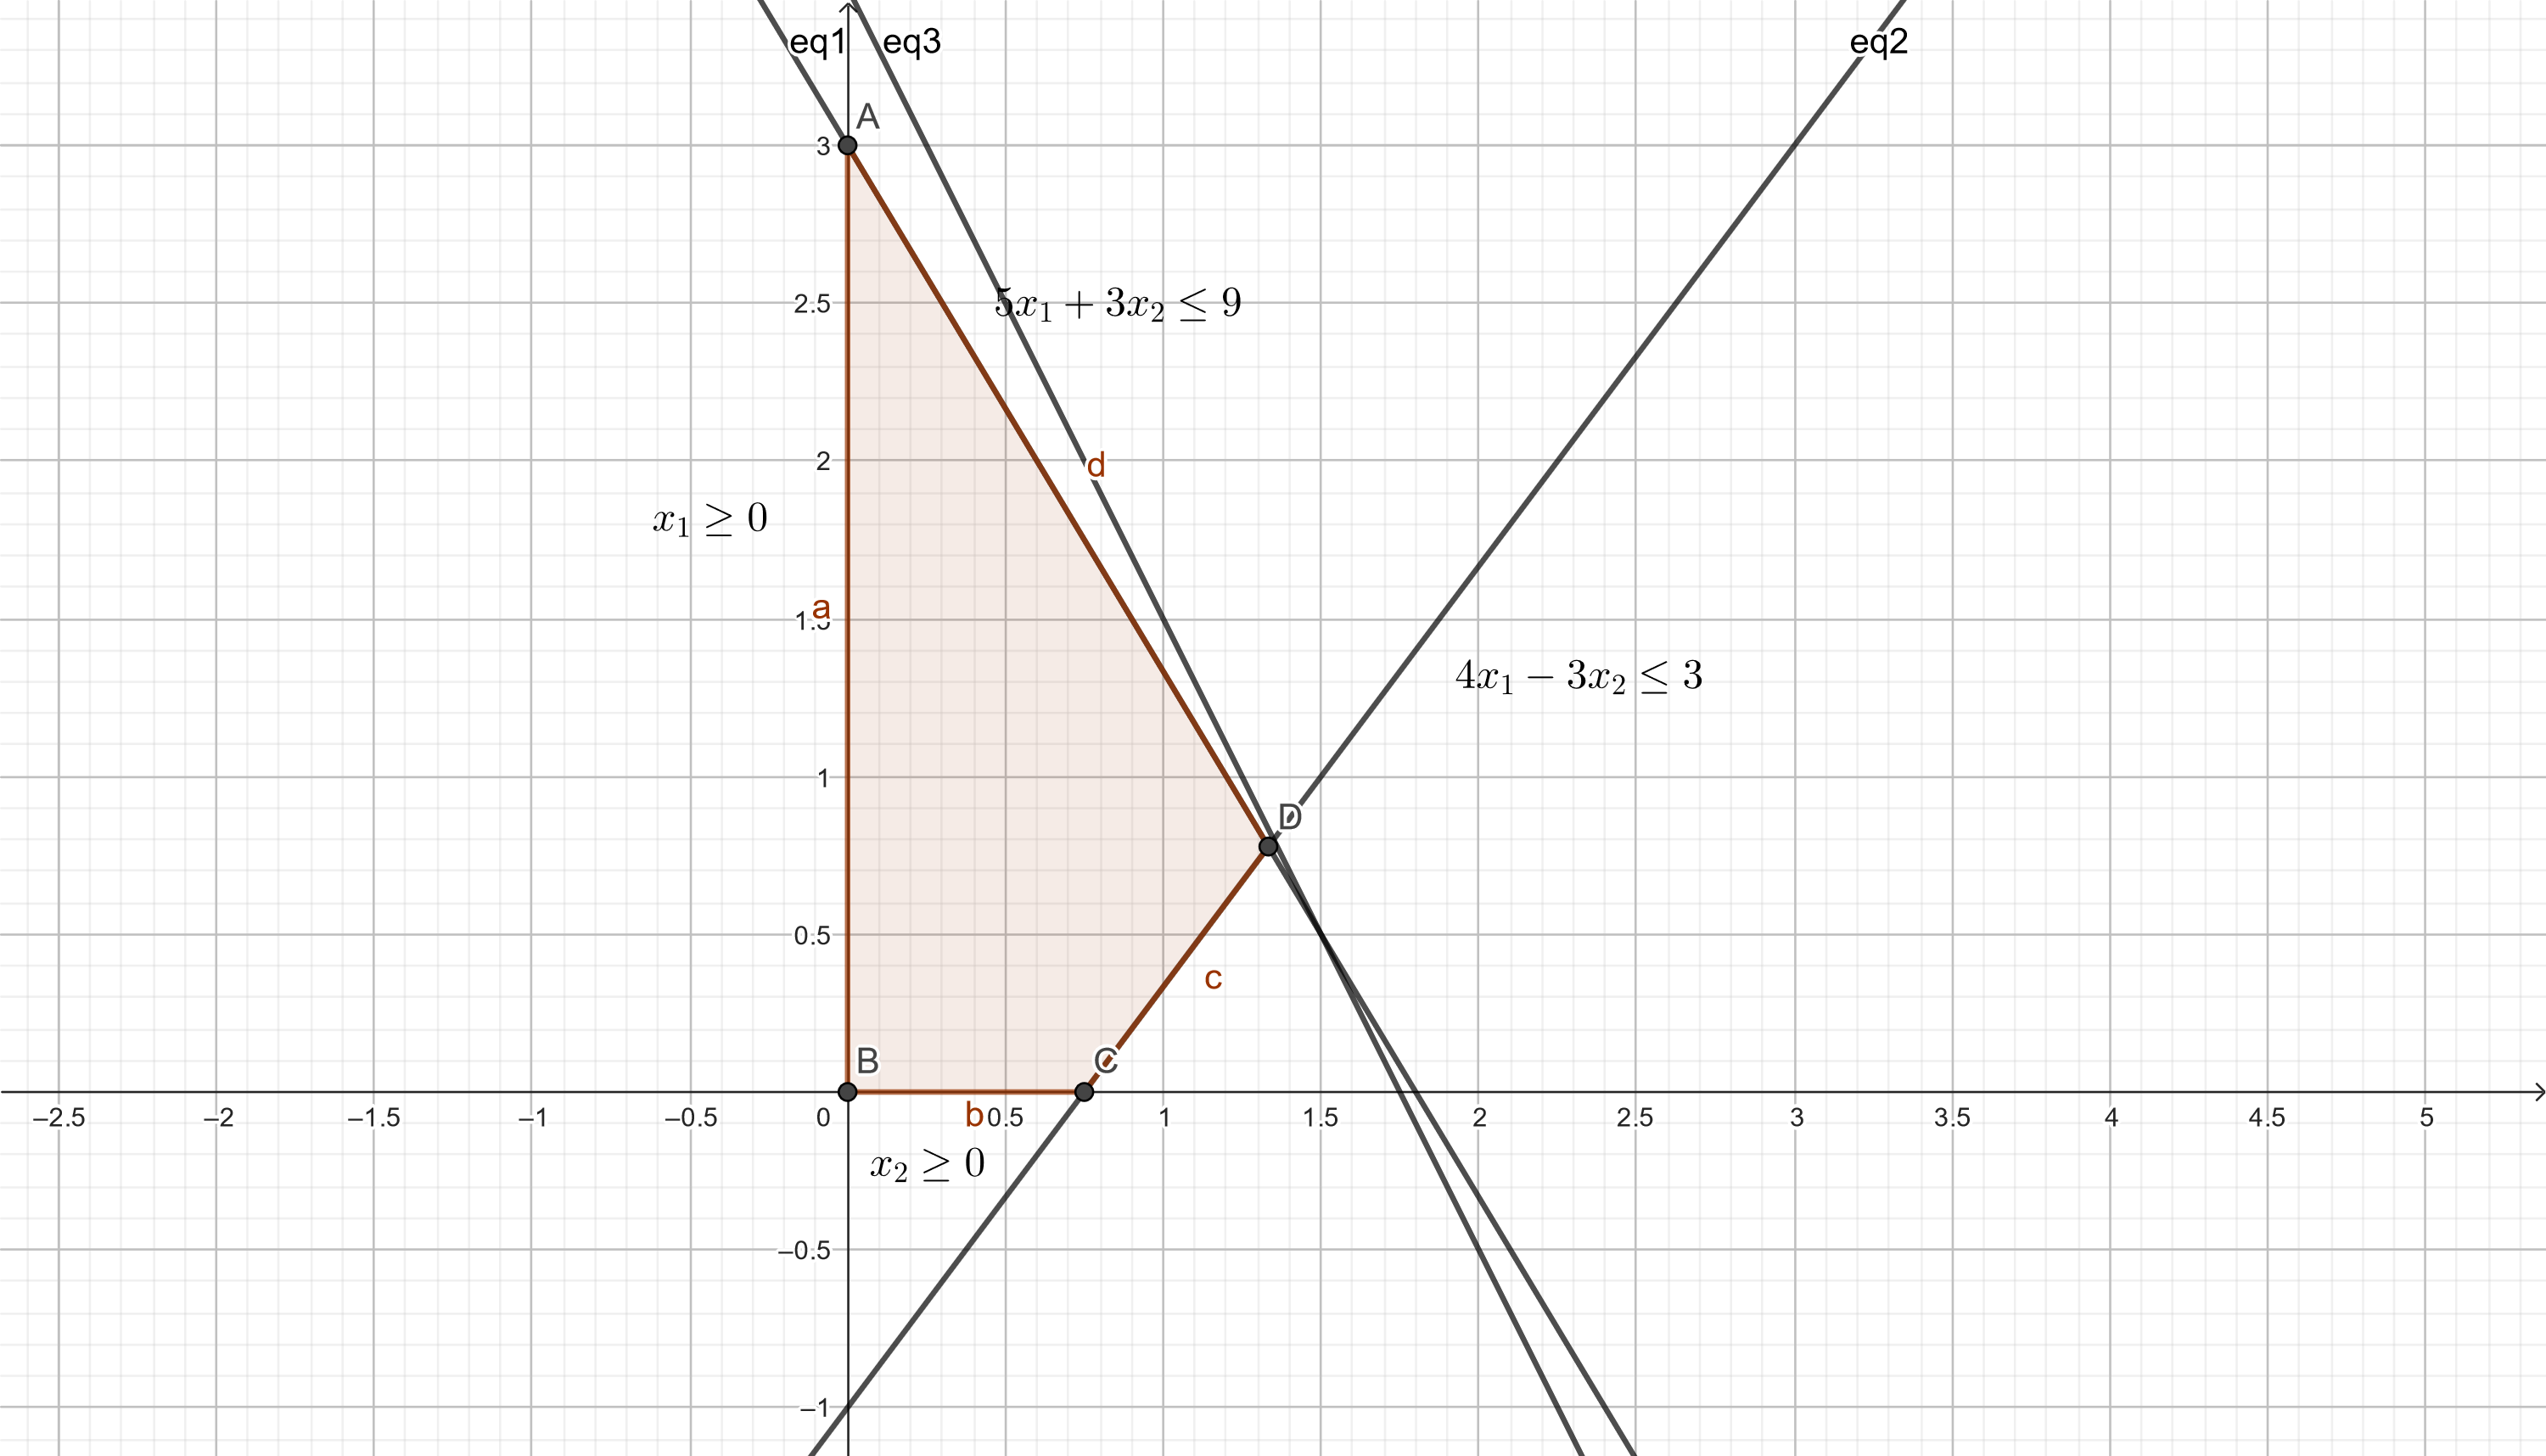
\includegraphics[width=12cm]{ass3-1.png}
\end{center}

Dopo aver disegnato i vincoli sul grafico si ricava il valore ottimo del rilassamento continuo, coincidente con il punto D. Quindi il primo nodo avra' $x_1=1.33,x_2=0.78$ e $Z_1=3.44$.
Seleziono arbitrariamente $x_1$ e applico il B\&B su di esso: $x_1 \leq \floor 1.33$ e $x_1 \geq \ceil 1.33$.

\begin{forest}
  for tree={
    circle,
    black,
    draw,
    fill=blue!30,
    s sep=20mm
  }
  [{$Z_1 = 3.44$},
    [{$Z_2 = ?$}, edge label={node[midway,below,font=\scriptsize]{$x_1 \leq 1$}}]
    [{$Z_3 = ?$}, edge label={node[midway,below,font=\scriptsize]{$x_1 \geq 2$}}]
  ]
\end{forest}

\newpage
\paragraph{Passo 2}
\begin{center}
        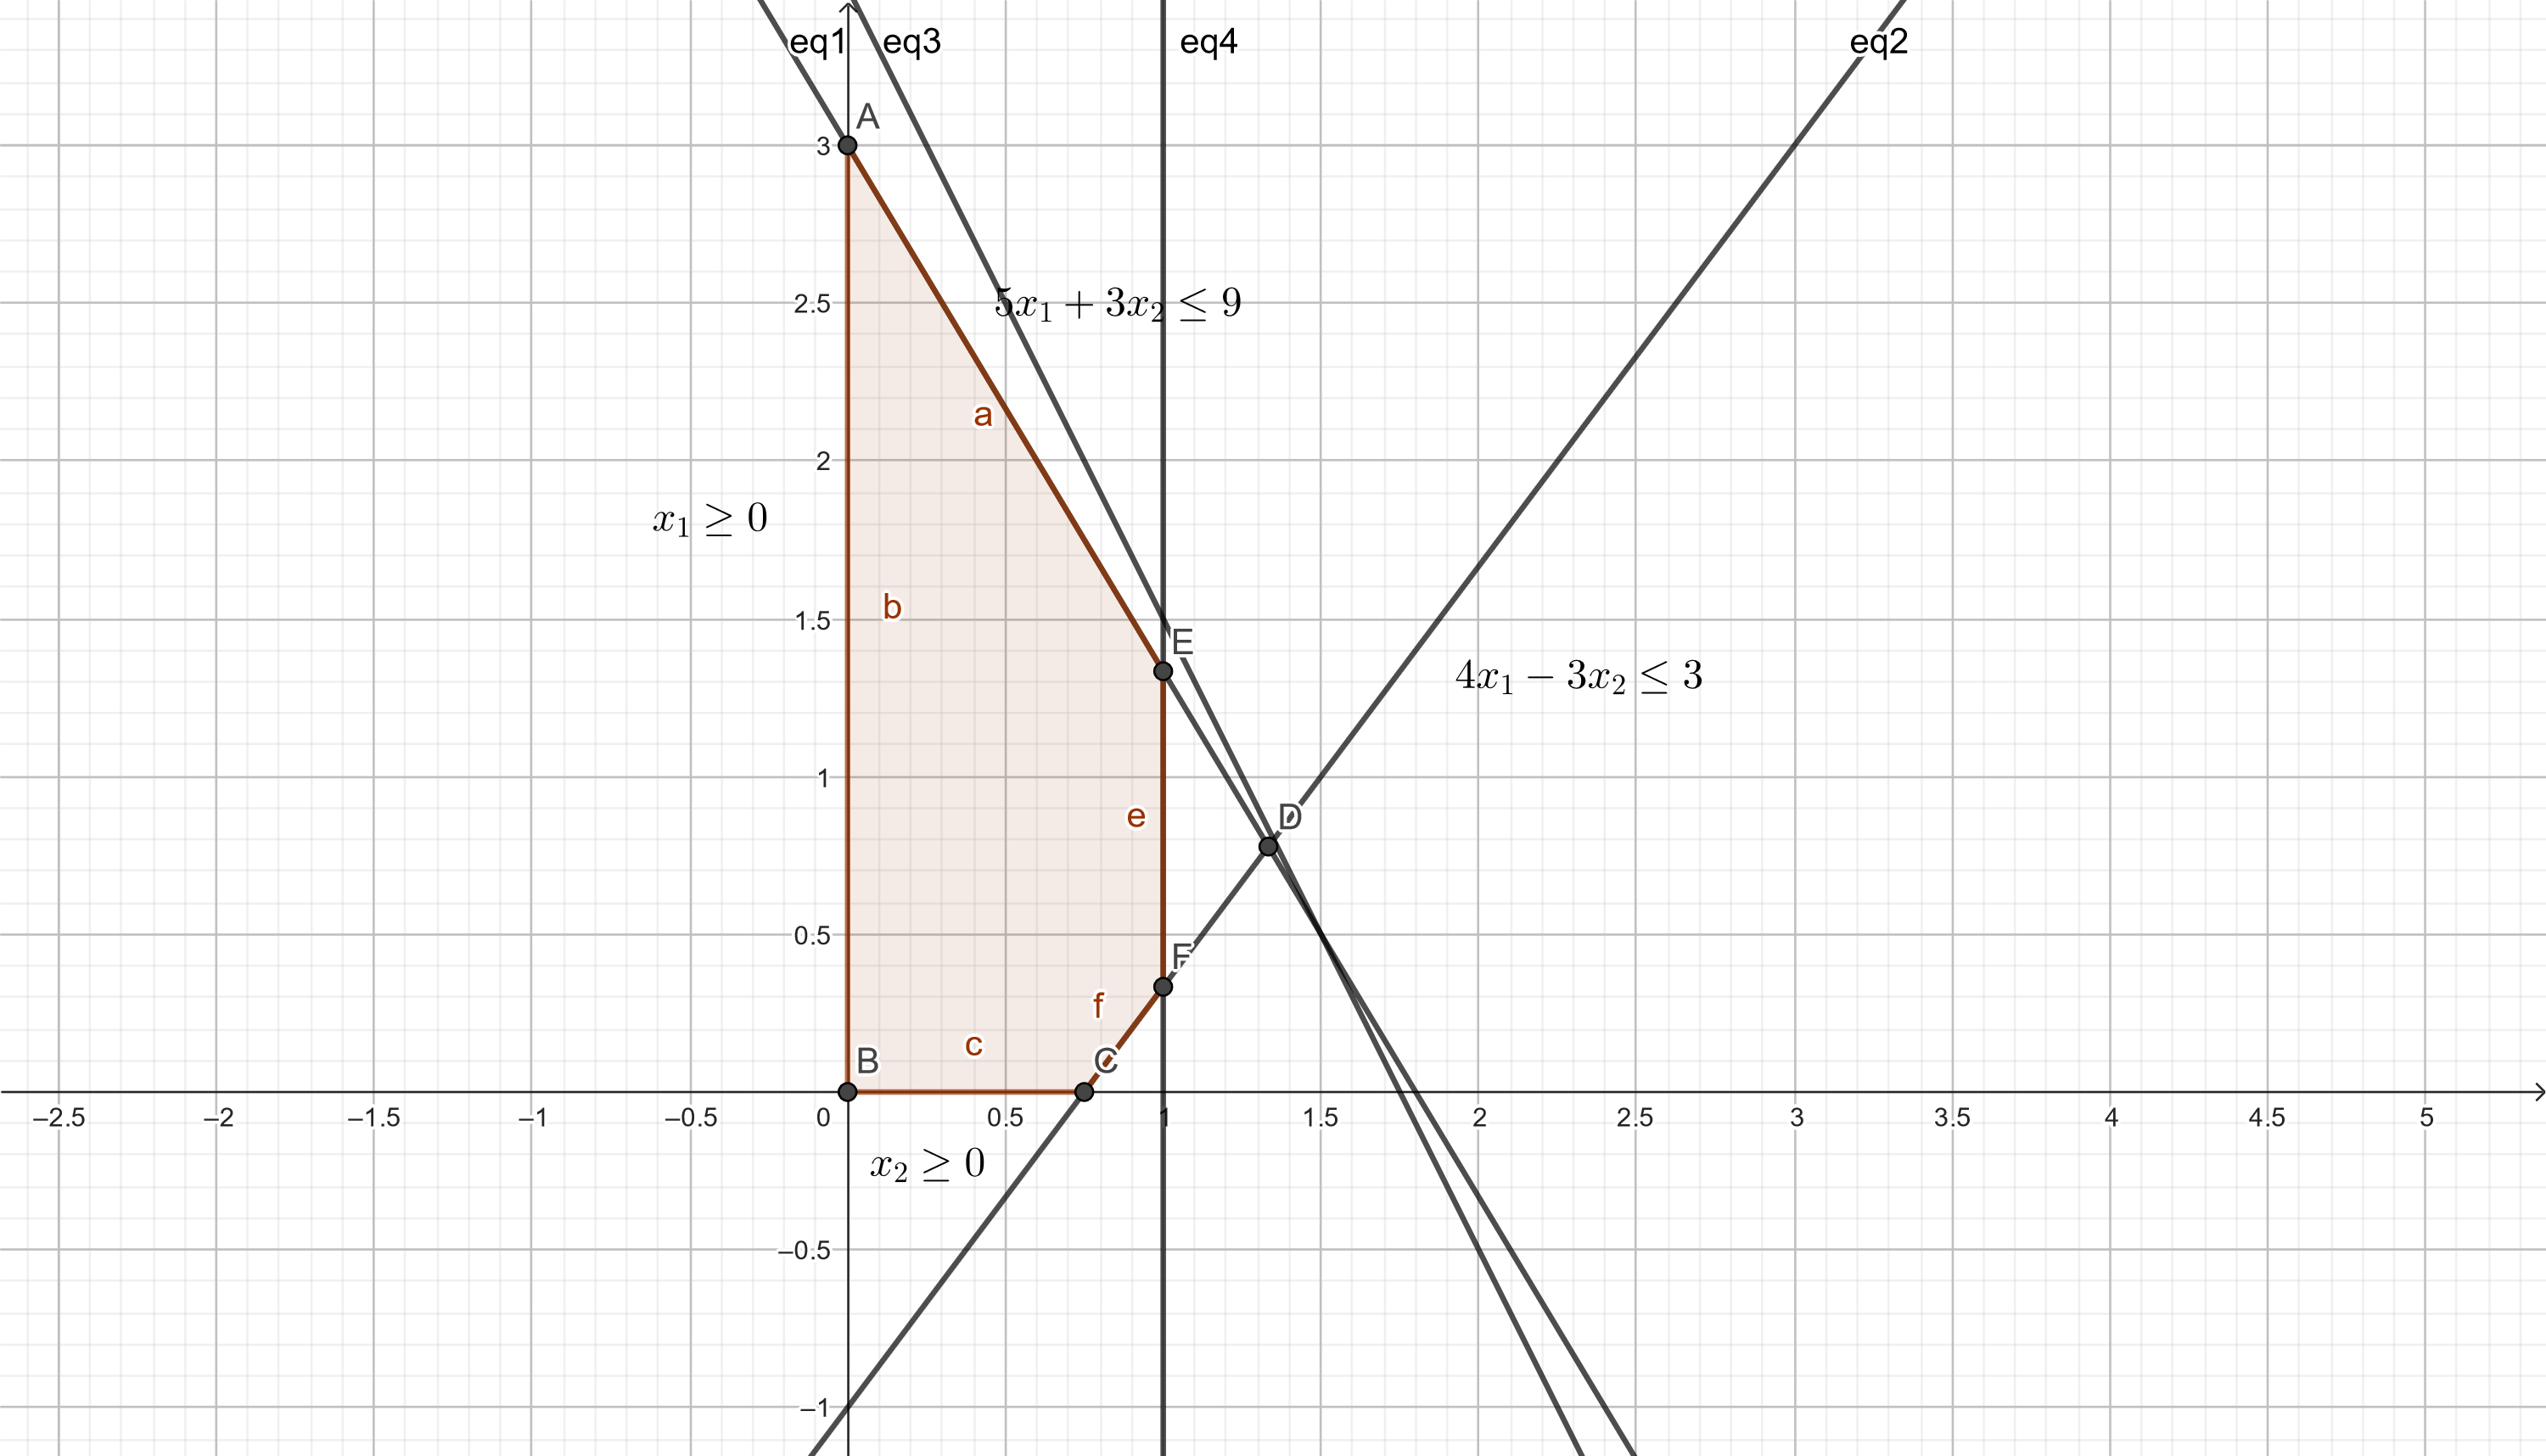
\includegraphics[width=12cm]{ass3-2.png}
\end{center}

Quindi navigo a sinistra e uso $x_1 \leq 1$. Dopo aver ridisegnato la regione ammissibile ottengo che il valore ottimo coincide con il punto E. Quindi questo nodo avra' $x_1=1, x_2=1.33$ e $Z_2=3.33$.
Seleziono quindi $x_2$ e applico il B\&B su di esso: $x_2 \leq \floor 1.33$ e $x_2 \geq \ceil 1.33$.

\begin{forest}
  for tree={
    circle,
    black,
    draw,
    fill=blue!30,
    s sep=20mm
  }
  [{$Z_1 = 3.44$},
    [{$Z_2 = 3.33$}, edge label={node[midway,below,font=\scriptsize]{$x_1 \leq 1$}},
      [{$Z_4 = ?$}, edge label={node[midway,below,font=\scriptsize]{$x_2 \leq 1$}}]
      [{$Z_5 = ?$}, edge label={node[midway,below,font=\scriptsize]{$x_2 \geq 2$}}]]
    [{$Z_3 = ?$}, edge label={node[midway,below,font=\scriptsize]{$x_1 \geq 2$}}]]
\end{forest}

\newpage
\paragraph{Passo 3}
\begin{center}
        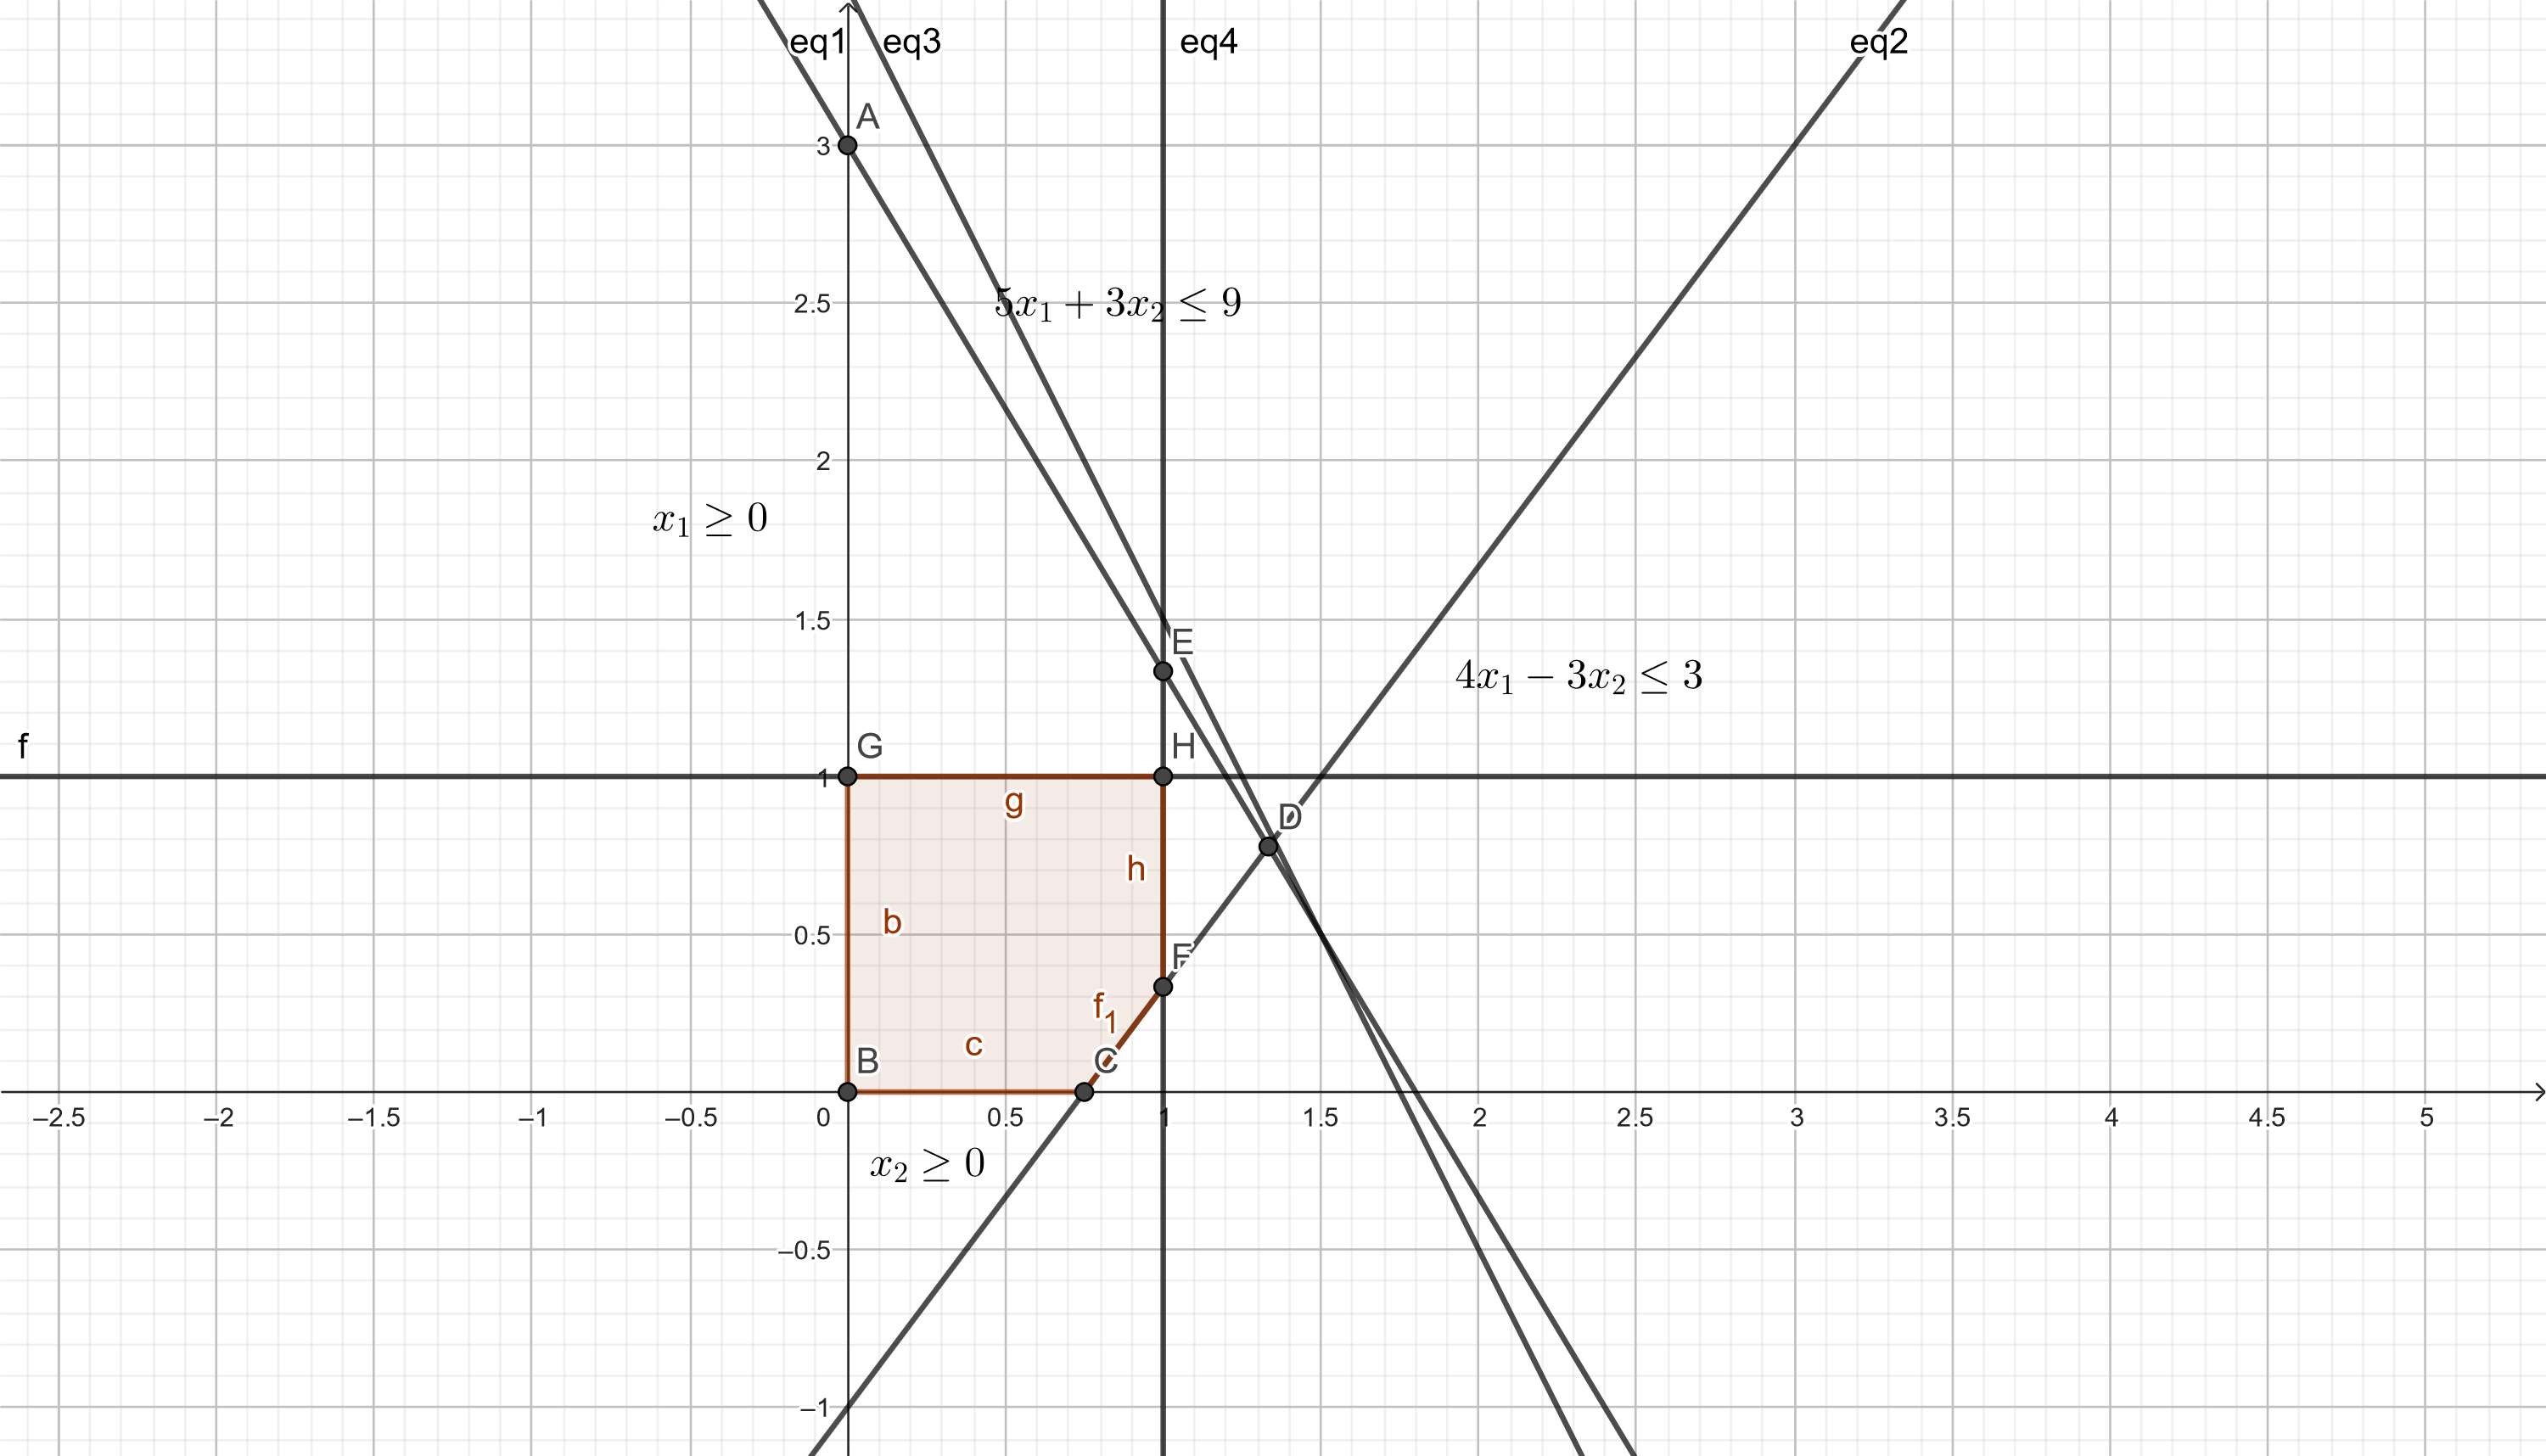
\includegraphics[width=12cm]{ass3-3.png}
\end{center}

Navigo a sinistra e uso $x_2 \leq 1$. Dopo aver ridisegnato la regione ammissibile ottengo che il valore ottimo coincide con il punto H. Quindi questo nodo avra' $x_1=1, x_2=1$ e $Z_4=3$.
E' una soluzione intera e ammissibile. L'esplorazione di questo sotto albero termina.

\begin{forest}
  for tree={
    circle,
    black,
    draw,
    fill=blue!30,
    s sep=20mm
  }
  [{$Z_1 = 3.44$},
    [{$Z_2 = 3.33$}, edge label={node[midway,below,font=\scriptsize]{$x_1 \leq 1$}},
      [{$Z_4 = 3$}, edge label={node[midway,below,font=\scriptsize]{$x_2 \leq 1$}}]
      [{$Z_5 = ?$}, edge label={node[midway,below,font=\scriptsize]{$x_2 \geq 2$}}]]
    [{$Z_3 = ?$}, edge label={node[midway,below,font=\scriptsize]{$x_1 \geq 2$}}]]
\end{forest}

\newpage
\paragraph{Passo 4}
\begin{center}
        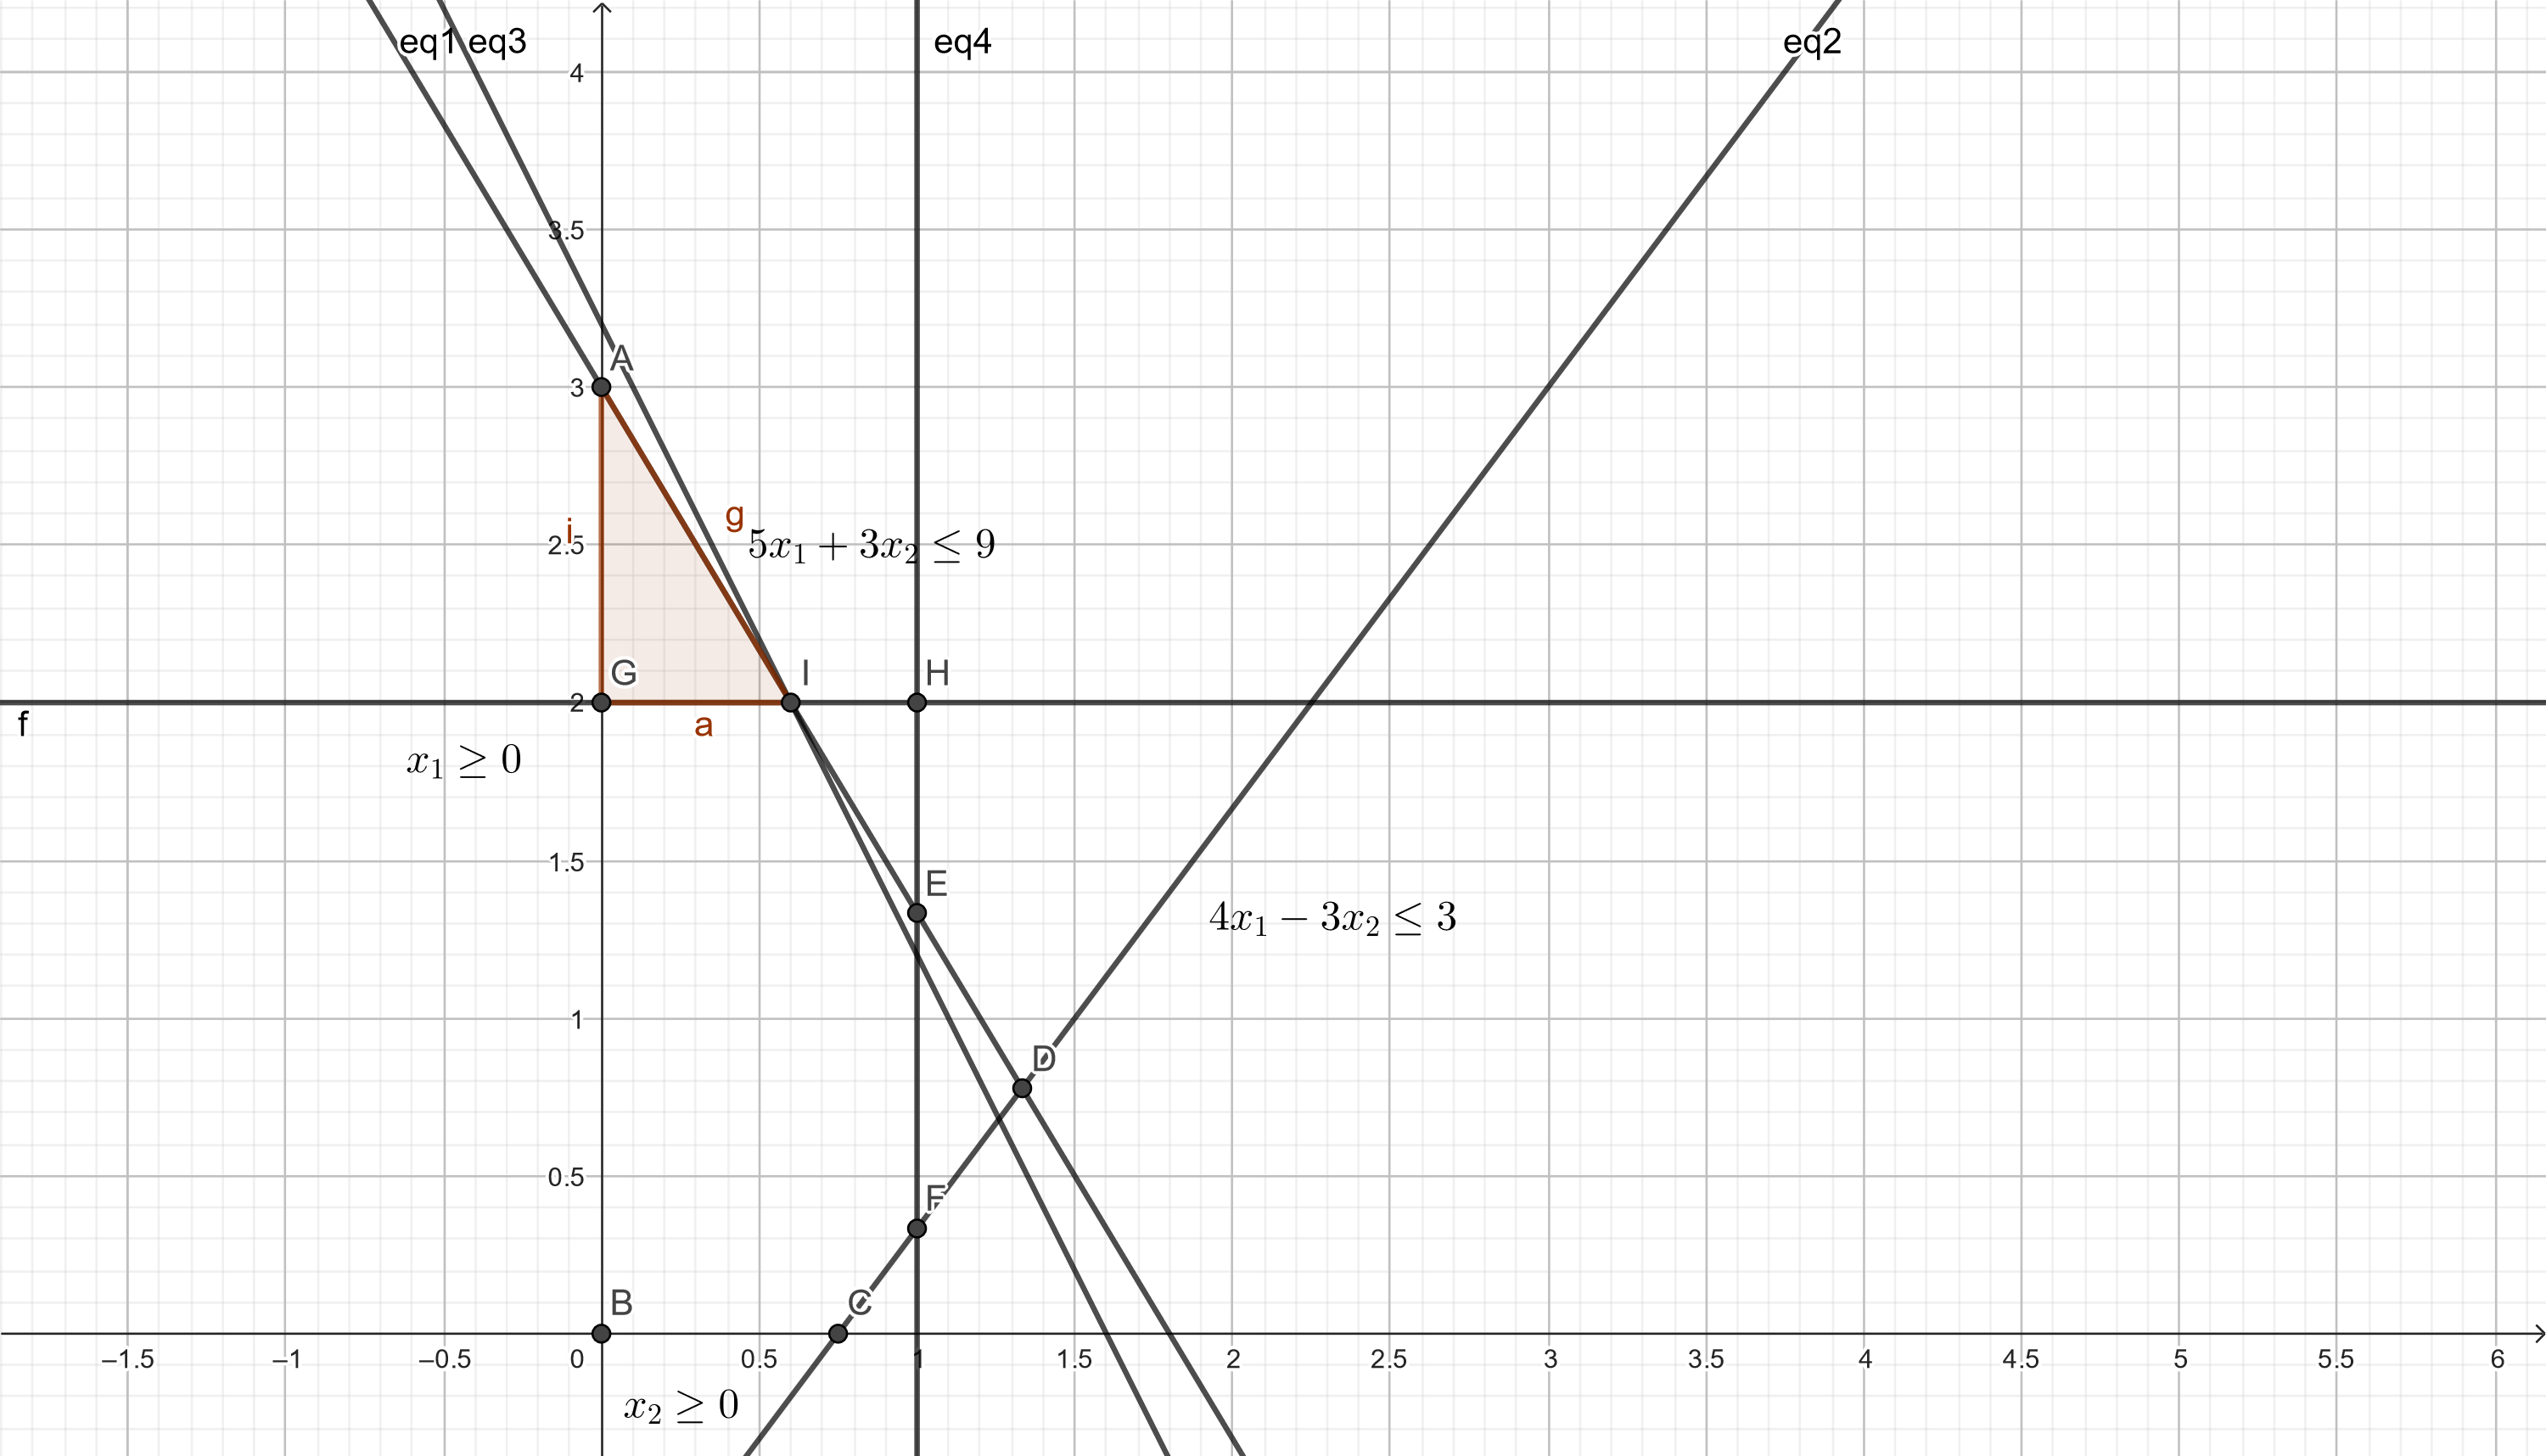
\includegraphics[width=12cm]{ass3-4.png}
\end{center}

Tornato al problema padre, navigo a destra in $x_2 \geq 2$. Dopo aver ridisegnato la regione ammissibile ottengo che il valore ottimo coincide con il punto I. Quindi questo nodo avra' $x_1=0.6, x_2=2$ e $Z_5=3.2$.
Tuttavia, esiste una soluzione intera e ammissibile $Z_4$ tale che $Z_4 \geq \floor Z_5$. Per bounding termino l'esplorazione del sottoalbero.

\begin{forest}
  for tree={
    circle,
    black,
    draw,
    fill=blue!30,
    s sep=20mm
  }
  [{$Z_1 = 3.44$},
    [{$Z_2 = 3.33$}, edge label={node[midway,below,font=\scriptsize]{$x_1 \leq 1$}},
      [{$Z_4 = 3$}, edge label={node[midway,below,font=\scriptsize]{$x_2 \leq 1$}}]
      [{$Z_5 = 3.2$}, edge label={node[midway,below,font=\scriptsize]{$x_2 \geq 2$}}]]
    [{$Z_3 = ?$}, edge label={node[midway,below,font=\scriptsize]{$x_1 \geq 2$}}]]
\end{forest}

\newpage
\paragraph{Passo 5}
\begin{center}
        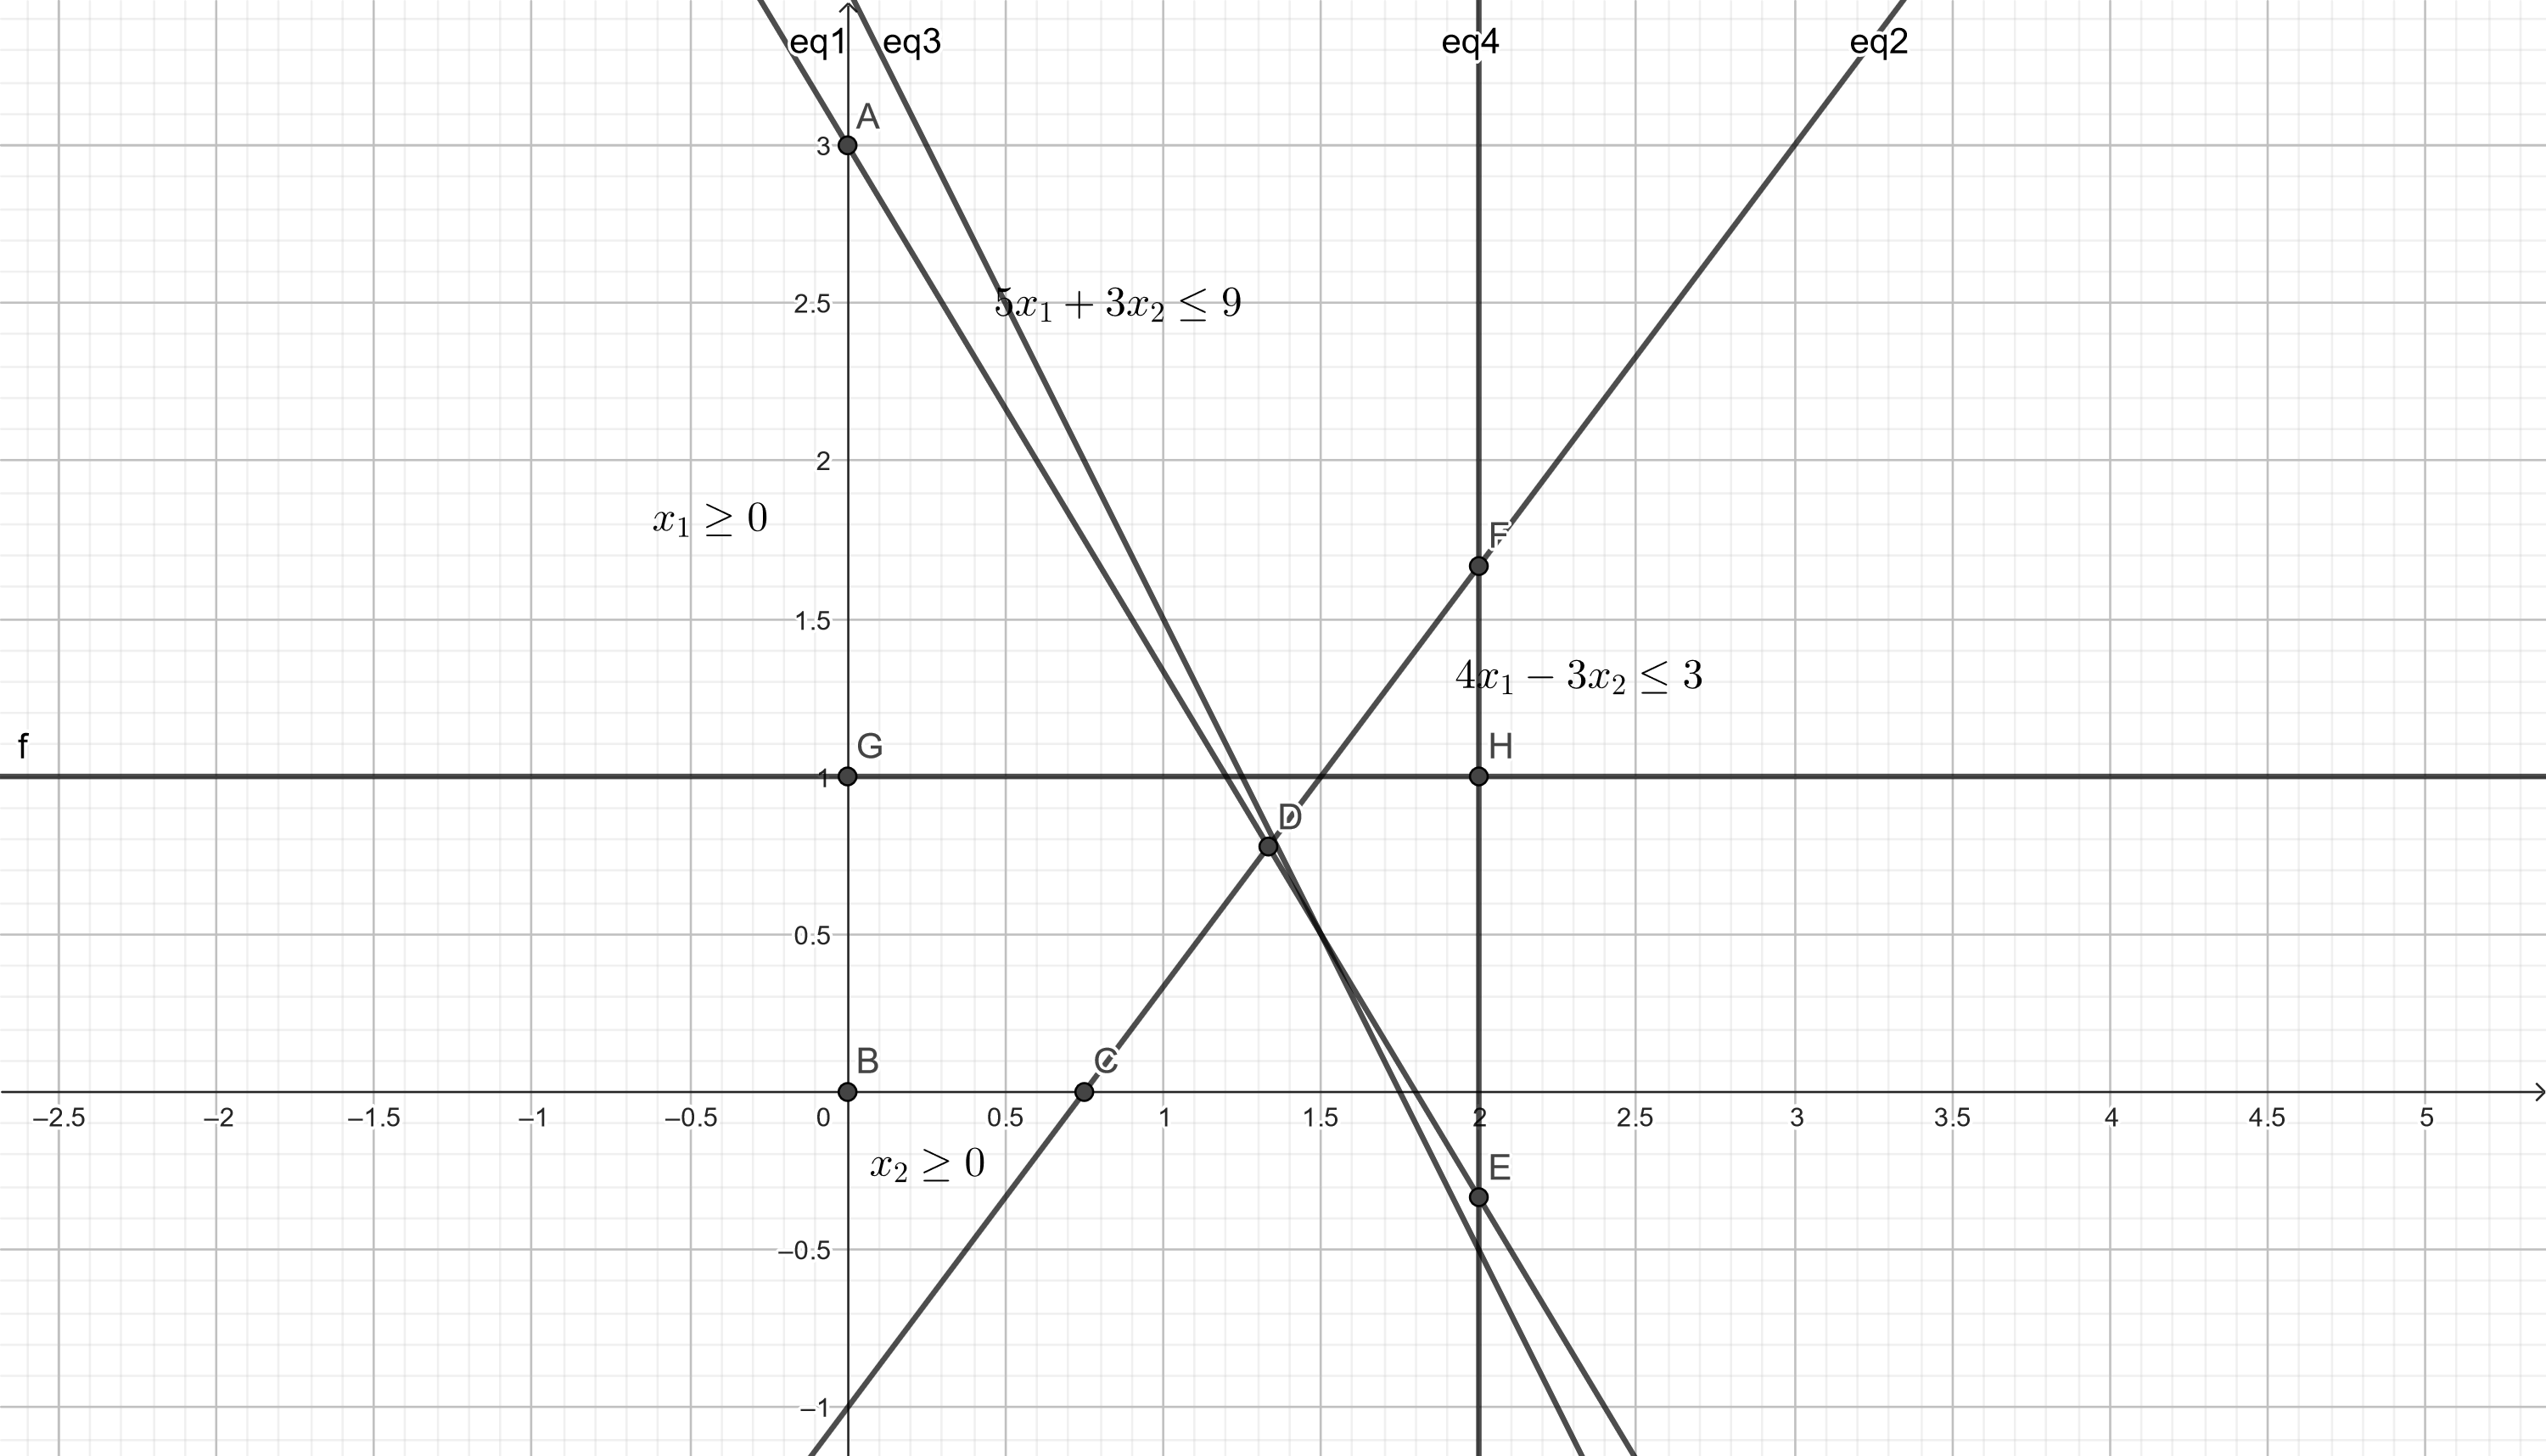
\includegraphics[width=12cm]{ass3-5.png}
\end{center}

Tornato al problema padre del problema padre, navigo a destra in $x_1 \geq 2$. Dopo aver ridisegnato la regione ammissibile ottengo la regione ammissibile e' vuota. Il problema corrente e' impossibile. Termino l'esplorazione del sotto albero.

\begin{forest}
  for tree={
    circle,
    black,
    draw,
    fill=blue!30,
    s sep=20mm
  }
  [{$Z_1 = 3.44$},
    [{$Z_2 = 3.33$}, edge label={node[midway,below,font=\scriptsize]{$x_1 \leq 1$}},
      [{$Z_4 = 3$}, edge label={node[midway,below,font=\scriptsize]{$x_2 \leq 1$}}]
      [{$Z_5 = 3.2$}, edge label={node[midway,below,font=\scriptsize]{$x_2 \geq 2$}}]]
    [{$Z_3 = IMP$}, edge label={node[midway,below,font=\scriptsize]{$x_1 \geq 2$}}]]
\end{forest}

Concludo che la soluzione ottimale intera per il problema dato e' $x_1=1, x_2=1$ con $Z=3$.

\end{document}
